\section{杂题}

\begin{frame}
\frametitle{CF744D Hongcow Draws a Circle}
\pause
平面上有n个红点和m个蓝点$(1 \le n,m \le 1000)$。

你要找一个半径最大的圆，使得它包含至少一个红点，并且不包任何一个蓝点。

如果答案可以无限大输出-1。

\pause
如何判-1？只要所有蓝点构成的凸包没有包含(不能在边界上)所有红点则无解。

\pause
如果有解，那么最大的圆上一定有一个蓝点(否则可以继续把圆扩大)
\end{frame}

\begin{frame}
\frametitle{CF744D Hongcow Draws a Circle}
\framesubtitle{方法一}
\pause
二分答案mid，然后枚举所有的蓝点k。

对每一个点都画一个半径为mid的圆。

如果某个圆和k有交，那么在交的哪一段极角区域打上标记。

然后做一遍扫描线，判断是否存在某个极角区域只有红标记没有蓝标记。

\textbf{pay \ atttention:}直接二分答案是不满足单调性的，因为把半径加长可能导致与蓝点相交，把半径缩短可能导致无法连接到红点。所以我们需要找到能连接到红点的最短距离。那么我们先对所有的红点为中心做一次二分答案，求出红点在圆上时半径最大值。然后再以蓝点为中心进行二分答案，以红点得到的答案为下界，这样答案就是满足单调性的了。
\end{frame}

\begin{frame}
\frametitle{CF744D Hongcow Draws a Circle}
\framesubtitle{方法二}
\pause
枚举了蓝点k之后，我们要找一个经过点k，包含至少一个红点，且不能包含蓝点的圆。

考虑反演，过k点的圆反演之后变成了一条直线，圆内的点就是直线外侧的点。

圆的半径和直线到k的距离成反比，所以我们需要最小化直线到k的距离。

\pause
分析一下可以发现，最优直线一定是蓝点构成的凸包上的边。

那么我们枚举完k之后构出反演之后的凸包，然后枚举凸包上所有边，再$O(n)$判断一下这条直线外侧是否有红点。

看起来复杂度是$nm^2$的，但是我们可以构出原图中蓝点的三角剖分。对于点k而言，只有在三角剖分中与点k有边的点才会出现在反演后的图的凸包中。所以复杂度是$n*$三角剖分边数总和的。注意到三角剖分是一个平面图，所以边数是线性的。
\end{frame}

\begin{frame}
\frametitle{清华集训2016 定向越野}
\pause
平面上有n个圆，互相之间不相交。

要从平面上一个点到达另一个点，不能经过任何圆盘内部。求最短路。

$n \le 500$

\end{frame}

\begin{frame}
\frametitle{清华集训2016 定向越野}
\pause
最终路径一定是若干条圆与圆之间的公切线和若干段圆周连接而成。

\pause
求与其他圆不相交公切线，构图。

\pause
求最短路(根据题目特性对于每个圆做特殊处理)。

\pause
可以暴力构图，$O(n^2)$枚举所有公切线，$O(n)$检验一条公切线是否穿过了其它圆。

\pause
可以用扫描线优化到$O(n^2logn)$
\end{frame}

\begin{frame}
\pause
给定平面上的n个点，求它们的欧几里得最小生成树

$n \le 10^5$

\pause
构出三角剖分，做最小生成树。
\end{frame}

\begin{frame}
\frametitle{CF536 C Tavas and Pashmaks}
\pause
题目大意:$n$个人比赛，要游泳$Sm$，跑步$Rm$(S,R未知),已知每个人的$V_s,V_r$,求所有可能取胜的人

\pause
我们把一个人看成平面上一个点$(\frac{1}{V_s},\frac{1}{V_r})$。那么一个人花费的时间就是与$(S,R)$的点积。

很显然，点集中与某个向量点积最大的点一定位于凸包上。

我们构出凸包，然后输出从横坐标最小的点到纵坐标最小的点这一段。
\end{frame}

\begin{frame}
\frametitle{cyclotron}
\pause
给你N个不经过原点的圆。让你求一个过原点的圆，使得与它有交点的圆尽量多。（所求的圆可以退化为直线）$N \le 1000$

\pause
以原点为中心反演，那么现在问题变成了：求一条直线使得与它有交点的圆尽量多。

\pause
很显然答案一定可以与两个圆相切(否则可以把直线进行偏转)

枚举一个圆，然后求出其它圆和这个圆相切对应的极角范围，然后扫描线即可。
\end{frame}

\begin{frame}
\frametitle{Codechef QPOINT}
\pause
在二维平面内，给定n个没有公共点的简单多边形。每次询问一个点，回答这个点属于哪个简单多边形，强制在线。

$n \le 10^5$，简单多边形的顶点数之和$\le 3*10^5$，询问个数$\le 10^5$。

\pause
裸题。

先特判在一条竖线上的情况，其余的直接做可持久化扫描线。
\end{frame}

\begin{frame}
\frametitle{圆的面积并}
\pause
求n个圆的并的面积$(n \le 1000)$

\pause
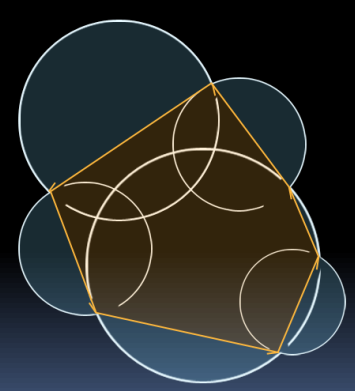
\includegraphics[height=4cm]{geometry/bing.png}

如图，最后形成的图形是由很多弓形和多边形组成的。

弓形的面积可以单独计算，多边形的面积可以用叉积算。
\end{frame}

\begin{frame}
\frametitle{圆的面积并}
\pause
如图，对于每个圆，用其它的圆与之求交，找到所有没有被覆盖的圆弧。圆弧须以逆时针序表示。

对于每条圆弧，累加其弓形的面积，以及这条边的有向面积。

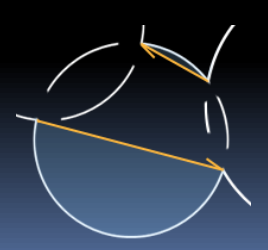
\includegraphics[height=5cm]{geometry/bing2.png}
\end{frame}

\begin{frame}
\frametitle{圆的面积并}
\framesubtitle{有洞？}
\pause
由于我们用的是叉积-有向面积，所以洞会被自动抵消。

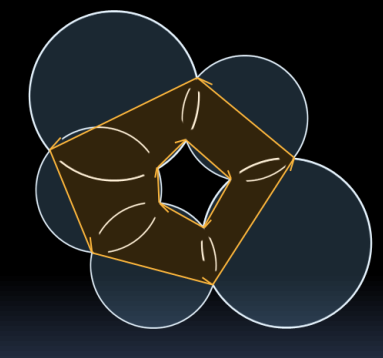
\includegraphics[height=6cm]{geometry/bing6.png}
\end{frame}

\begin{frame}
\frametitle{最小圆}
\pause
求解包含某个点集的半径最小的圆

\pause
很显然，最终的圆一定会被边界点卡住而无法向任何方向平移。

\pause
要卡住一个圆，要么是一对点$(a,b)$，满足圆心在直线AB上，要么是三个不相同的点$(a,b,c)$。

\pause
所以我们枚举点a，如果存在点b到a的距离大于当前答案则把圆心设为ab中点，半径为$\frac{|ab|}{2}$，再枚举点c,如果c到圆心的距离大于$\frac{|ab|}{2}$则把圆心切换为abc的中点。
\end{frame}

\begin{frame}
\frametitle{判断两个多边形的交面积是否$>0$}
\pause
Case \ 1:有两条线段严格相交(一条线段上的点不允许在另一条直线上)

直接叉积判断即可

\pause
Case \ 2:有一个点在另一条线段上。

判断这个点相邻的两个点是否分布两侧

\pause
Case \ 3:有两个点相同

判断这两个点相邻一共四个点的位置关系。
\end{frame}

\begin{frame}
\frametitle{POJ3675}
\pause
求多边形和圆的交

\pause
看起来非常复杂，但是我们可以把多边形拆成若干个三角形分别计算。

利用叉积的方向，我们可以取任意点为基准点，自然取圆心最方便计算。

\pause
现在的任务就是计算一个以原点为圆心，半径为R的圆和$\triangle ABC$的交面积。
\end{frame}

\begin{frame}
\frametitle{POJ3675}
\framesubtitle{Case 1}
\pause
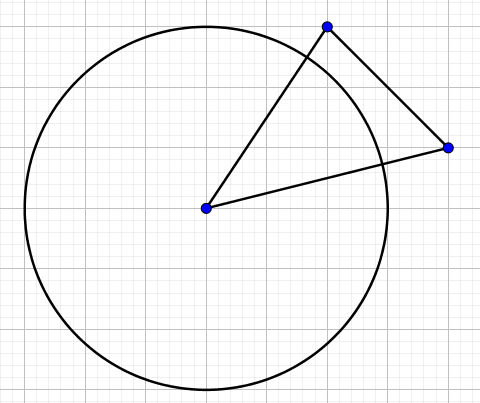
\includegraphics[height=5cm]{geometry/case1.png}

线段AB完全在圆外

面积就是一段扇形的面积。
\end{frame}

\begin{frame}
\frametitle{POJ3675}
\framesubtitle{Case 2}
\pause
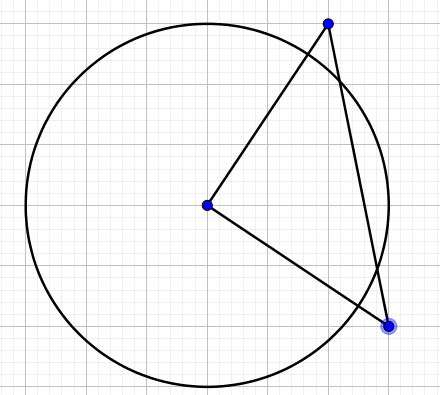
\includegraphics[height=5cm]{geometry/case2.png}

点AB完全在圆外，但是线段AB与圆有交

\pause
两段扇形+一个三角形
\end{frame}

\begin{frame}
\frametitle{POJ3675}
\framesubtitle{Case 3}
\pause
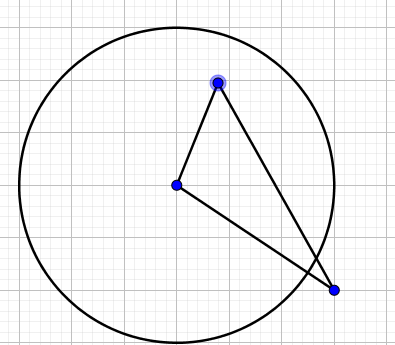
\includegraphics[height=5cm]{geometry/case3.png}

AB一个在圆外一个在圆内

\pause
一个扇形+一个三角形
\end{frame}

\begin{frame}
\frametitle{POJ3675}
\framesubtitle{Case 4}
\pause
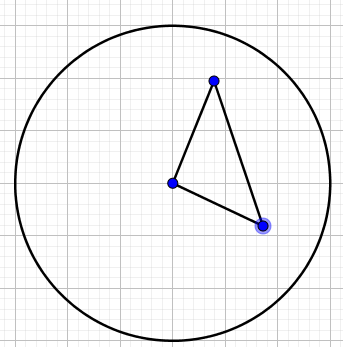
\includegraphics[height=5cm]{geometry/case4.png}

AB都在圆内

\pause
面积就是$S_{\triangle}ABC$
\end{frame}

\begin{frame}
\frametitle{清华集训2012Day4T3 阳光}
\framesubtitle{题目描述}
\pause
为了督促同学们长跑，体育组制作了“阳光长跑卡”，并要求同学们通过刷卡来证明自己跑过的距离。为了防止同学抄近路，体育组又在跑到上设置了很多个刷卡点，要求同学们依次刷过。为了防止同学互相代替刷卡，体育组便安排了一个老师在现场监督。然而，老师的视野范围有限，可能无法监督到所有的刷卡点。为了解决这一问题，体育组的老师来向你寻求帮助。

简要地说，我们可以把跑道看做一个以原点为圆心、半径为r的圆。监督的老师站在原点处，视野范围为一个给定的n边形，且顶点顺序满足以原点为中心的极角序。现让你在跑到上放置m个等距的刷卡点，使得尽可能多的刷卡点落在老师的视野范围内(视野范围包含多边形边界)。
\end{frame}

\begin{frame}
\frametitle{清华集训2012Day4T3 阳光}
\framesubtitle{sol}
\pause
首先求出圆上哪些区域被多边形覆盖，可以用$O(n)$段极角区间来表示。\newline \newline

\pause
我们的任务是确定一个量$d \in [0,\frac{2 \pi}{m})$，然后把把所有的刷卡点放在$k*\frac{2 \pi}{m}+d$上。\newline \newline

\pause
用点事件可以做到$nlogn$
\end{frame}

\begin{frame}
\frametitle{world final 2017 Airport Construction}
\pause
给你一个$n$个点的多边形，求它的直径。

\pause
例:
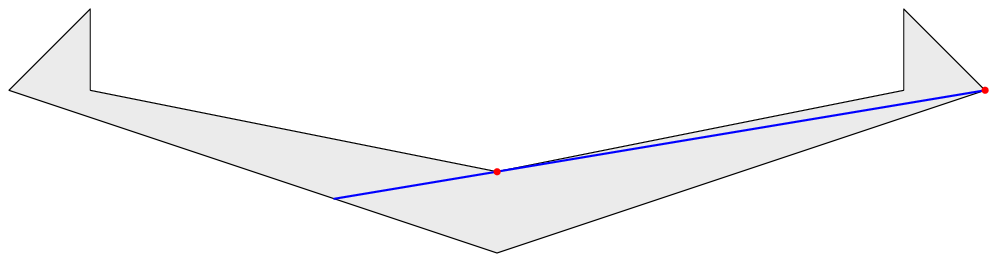
\includegraphics[height=3cm]{geometry/wf.png}

\pause
$n \le 200$

\pause
容易分析得出，直径一定至少经过其中两个点。否则可以调整变得更优。

可以先$n^2$枚举所有直线，然后判断在多边形内的最大线段长度。(难点)
\end{frame}

\begin{frame}
\frametitle{world final 2017 Airport Construction}
\framesubtitle{sol}
\pause
但是有很多种情况，稍微不注意可能就会挂。

\pause
\begin{multicols}{3}
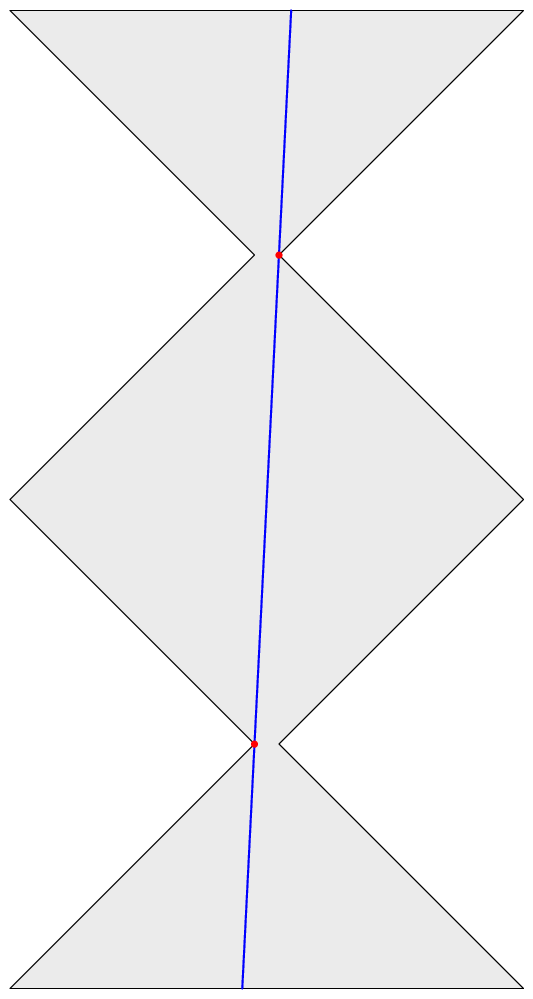
\includegraphics[width=3.5cm,height=3cm]{geometry/wf2.png}
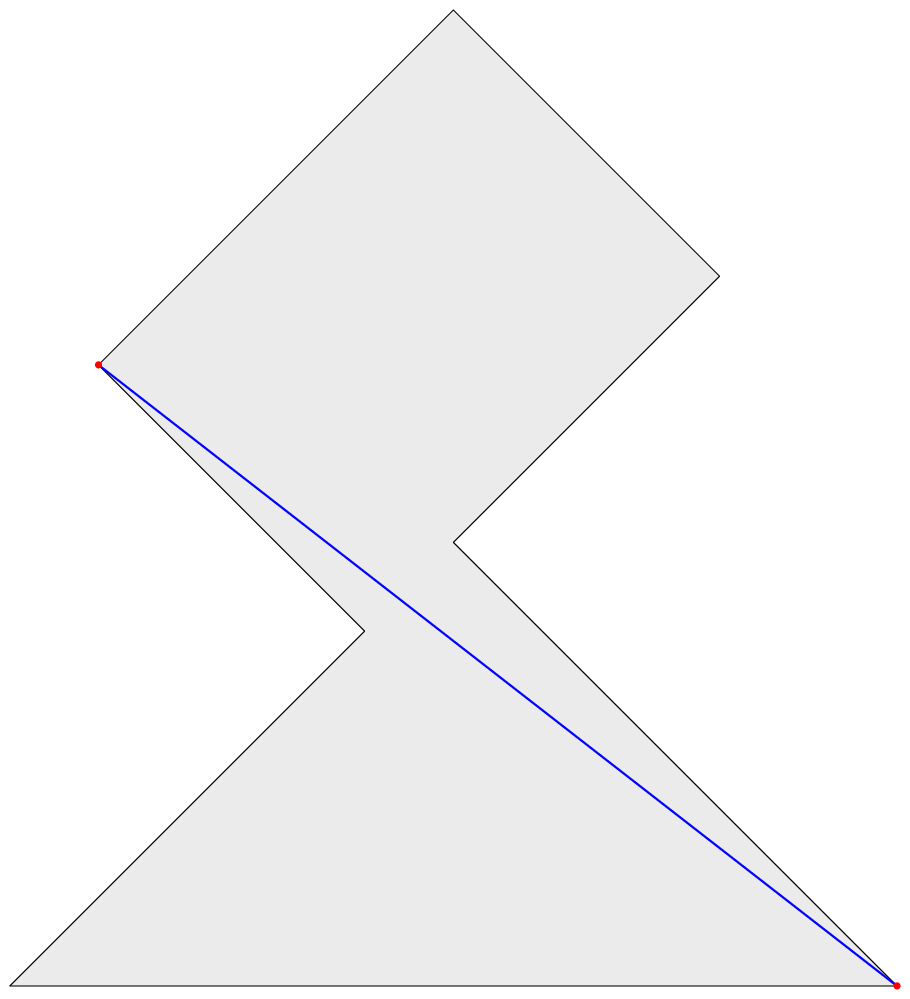
\includegraphics[width=3.5cm,height=3cm]{geometry/wf3.png}
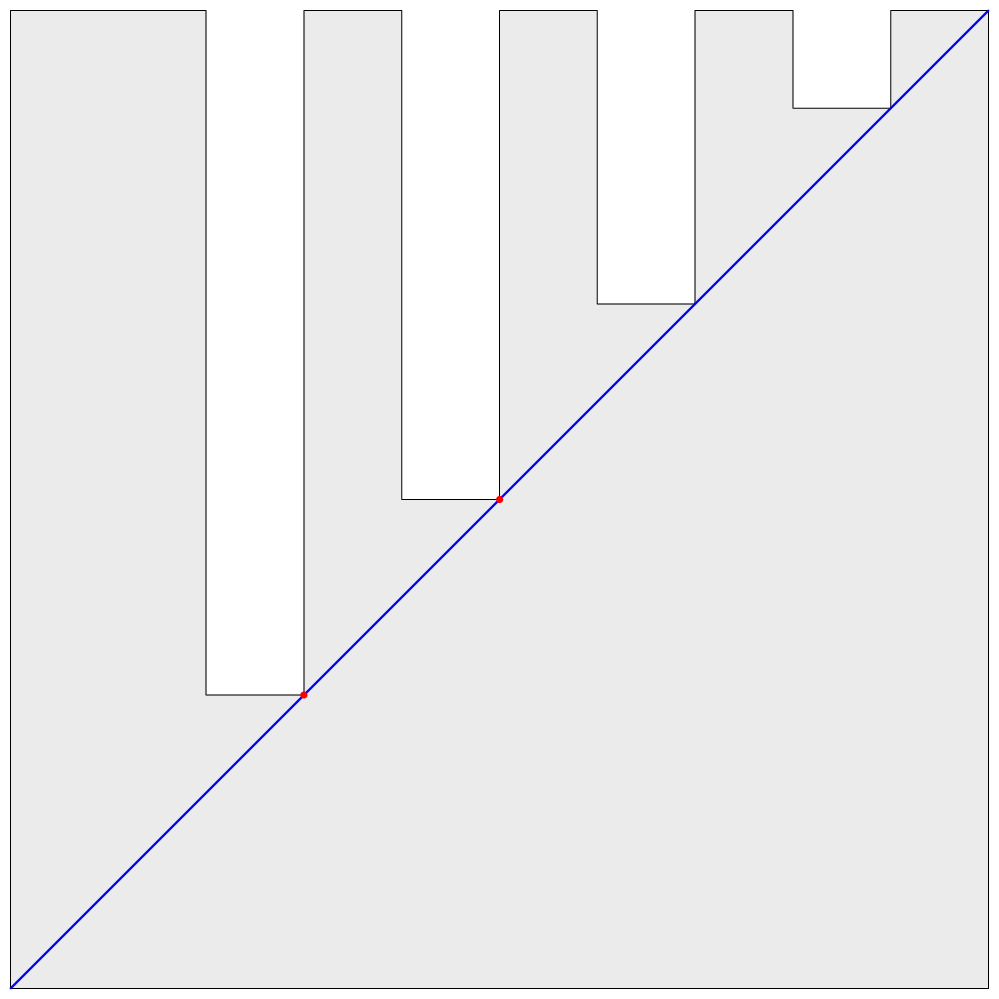
\includegraphics[width=4cm,height=3cm]{geometry/wf4.png}
\end{multicols}

\pause
而且还要特别注意的是：有可能枚举的直线都在多边形外。

这里推荐一种好写的方法：把直线和多边形的所有交点都记录到数组$cross[1 \cdots m]$中并排序，然后$cross[2k-1] \rightarrow cross[2k]$就是所有在多边形内部的区间。
\end{frame}

\begin{frame}
\frametitle{CTSC2017 投影}
\pause
k维空间中有n个黑点与n个白点。我们为每一个黑点确定一个互不相同的对应的白点，这样一共有$n!$种对应方法。我们定义这n个黑点与n个白点之间的“移动距离”为，在所有的对应方法中，对应的黑点与白点之间的 n个\textbf{欧几里德}距离的和的\textbf{最小值}。

你得到了三维空间中的n个黑点与n个白点。你想把它们投影到一个$k(1 \le k \le 2)$维子空间上。一维子空间就是三维空间中的一条直线，二维子空间则是三维空间中的一个平面。一个点在一个子空间中的投影点就是这个子空间中距离它最近的点。例如，$(0,0,0),(1,1,0),(1,0,0),(0,1,0)$这四个点投影到$x-y=0,z=0$这条直线上之后，得到的投影点是$(0,0,0),(1,1,0),(0.5,0.5,0),(0.5,0.5,0)$。

求着n个黑点和n个白点投影到k维子空间之后移动距离最大值。
\end{frame}

\begin{frame}
\frametitle{CTSC2017 投影}
\framesubtitle{30分：二维投影一维}
\pause
如果已知投影直线，求答案是非常轻松的。

按照在直线上的投影坐标排序，按照顺序匹配一定保证最优。(这个很好理解，交叉匹配不可能使答案更优)

\pause
如果在某段极角范围内，点在直线上的投影坐标相对顺序不变，则我们可以列出移动距离关于极角的函数，然后求得最值。

如果$A,B$投影坐标相对顺序发生变化，则发生变化的时刻为投影直线垂直于直线$AB$。

发生变化的事件个数为$O(n^2)$，扫描线找到所有区间，对这$O(n^2)$个区间分别求解。

\pause
现在的关键问题是，如果找到最优极值点。
\end{frame}

\begin{frame}
\frametitle{CTSC2017 投影}
\framesubtitle{30分：二维投影一维}
\pause
我在考场上想出一个做法，如果直线的极角为$\alpha$，一组匹配点的极角为$\beta$，欧几里得距离为d，则他们在直线上投影距离为$d \cos(\alpha-\beta)$

用三角函数公式，可以把所有匹配点的投影距离之和表示成$a\sin(\alpha)+b\cos(\alpha)$的形式。通过辅助角公式我们知道，这个函数可以通过一个三角函数的平移、拉伸得到，所以满足在跨度不超过$\pi$的一段区间，该函数为单峰函数，可以用三分法求得极值。\pause 复杂度为$O(n^2 \log n)$。\newline \newline

\pause
然而遗憾的是，$\cos$函数应该取绝对值，否则如果极角差$> \frac{\pi}{2}$则会爆负数。。。QAQ，然后我就愉快地爆零了。
\end{frame}

\begin{frame}
\frametitle{CTSC2017 投影}
\framesubtitle{30分：二维投影一维}
\pause
所以还要加上改动：对于一组匹配点$(a,b)$，在极角转过$\frac{\pi}{2}$之后要切换三角函数的符号。

每次修改函数值时，都要根据当前极角区间调整三角函数的符号。

\pause
std用了更优的方法。

对于所有的匹配$(a_i,b_i)$，我们统计出$(X,Y)=\sum_{i=1}^{n} (x_{b_i}-x_{a_i},y_{b_i}-y_{a_i})$

然后移动距离为$(X,Y)$在极角方向上的投影。那么显然极角方向离$(X,Y)$越近越好，根据左右边界范围可以$O(1)$求出最优解。

复杂度$n^2\log n$，不过这里的$\log$仅仅是排序，所以比我的方法快多了。

\pause
这个方法也要注意，当极角转过$\frac{\pi}{2}$后要切换为相反向量。
\end{frame}

\begin{frame}
\frametitle{CTSC2017 投影}
\framesubtitle{100分}
\pause
std的代码太繁杂了，这里就不多介绍。

\pause
xmk的做法是比较值得提倡的。

他用的是模拟退火算法，一开始随机一些平面法向量，然后求出在这些法向量下的移动距离。然后每次以一定概率接受附近的点。

如何求移动距离呢？投影到一维显然排序即可。投影到二维可以暴力一点使用二分图最大权匹配(KM \ or \ 费用流)。
\end{frame}

\begin{frame}{CF35E}
    给定$N$个下边界紧贴$X$轴，上边界在$X$轴上方的矩形 (矩形的四边都平行于坐标轴) 。
    
    求这个矩形的“轮廓”，即输出矩形的并的顶点坐标，要求轮廓相邻的边垂直。

    $N \le 10^5$
\end{frame}

\begin{frame}{CF35E}
    直观上来看，我们每次沿这边界行走，就能得到最后的答案，但是这样处理起来比较复杂。
    
    用另外一种更为简单的思路，我们将最后轮廓中所有的横向线段找出来，再把他们连接起来即可。
    
    考虑某个横坐标所对应的轮廓的纵坐标，实际上是覆盖它的所有横向线段中最高的那条。
    
    我们将所有的端点离散出来(因为转折点的横坐标只会在端点处产生) ，然后按横坐标从小到大依次扫描每个端点，同时维护当前的轮廓的纵坐标
    
    如果纵坐标发生了变化，则我们需要”拐弯”，将这个转折点记录下来即可。
    
    维护当前轮廓的纵坐标可以用系统堆。复杂度$O(n \log n)$。
    
\end{frame}

\begin{frame}{CF67E}

    给定一个简单多边形，第一条边一定平行于坐标轴，问第一条边上有多少个整点可以看到多边形上所有的顶点
    
    (看到的定义为连线段不会落在多边形外部)。

    数据范围: $n \le 1000,x_i,y_i \le 10^6$

    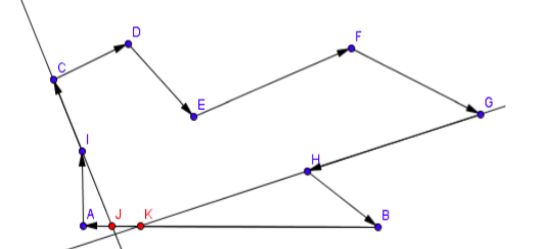
\includegraphics[width=10cm]{geometry/pG1.png}
\end{frame}

\begin{frame}
    我们规定以顺时针遍历所有的边，对于某条边$(a,b)$，它所在的直线的左边的点一定不能同时看到点$a$和$b$。
    
    所以通过这个我们可以在第一条边上加一个限制: 即只有在$(a,b)$所在直线的右边的点才是合法。最后我们对所有的限制取一个交即可。复杂度$O(n\log n)$。
\end{frame}

\begin{frame}
    给定一个凸多边形的三角剖分，从多边形的一个三角形出发，每次可以从一个三角形到其相邻的三角形，但是不能经过重复的三角形。
    
    问哪一对三角形之间的距离最长？

    $N \le 200000$
\end{frame}

\begin{frame}
    平面图的对偶图
    
    这是一棵树！
    
    树的最长链

\end{frame}

\begin{frame}
    给定平面上$n$个圆，问用$k$条线最多能将这$n$个圆分成多少份？

    $N \le 10^3, k \le 10^5$

\end{frame}

\begin{frame}
    若只有一个圆：$1 + K \times (K+1)/2$
    
    若有一条线穿过所有的圆：$1+K \times (K+1)/2+(N-1) \times (K+1)$
    
    希望找到一根线穿过的圆尽可能多
\end{frame}

\begin{frame}
    枚举这条线相切的一个圆（为什么相切？），

    我们可以用角度$[0,2 \pi]$来表示这条直线

    对于每个其它的圆，将会覆盖$[0,2 \pi]$中间的一段区间，然后查询被区间覆盖次数最多是多少次。$O(n\log n)$

\end{frame}

\begin{frame}
\frametitle{CF853E Lada Malina}
\pause
一辆汽车有k个引擎，每个引擎i有一个速度向量$(x_i,y_i)$。现在你可以给每个引擎一个\textbf{实数}参数$v_i \in [-1,1]$，那么汽车最终的速度向量为$(\sum v_ix_i,\sum v_iy_i)$

有n个工厂，i号工厂位于地点$fx_i,fy_i$，厂内有$a_i$辆汽车。

有q个展览会，每个展览会i会在地点$px_i,py_i$举行。每个工厂可以发车前往展览会。展览会$i$还有一个时间限制$t_i$表示汽车需要在$t_i$个单位时间内到达展览会。

求每个展览会最多可以有多少辆汽车在规定时间到达。

$2 \le k \le 10 \ \ 1 \le n,q \le 10^5 \ \ |vx_i|,|vy_i| \in [-1000,1000] \ \ |fx_i|,|fy_i|,|px_i|,|py_i| \le 10^9$
\end{frame}

\begin{frame}
    做法：由于$v_{i}$与$-v_{i}$等价，我们先把每个向量的横坐标变成非负（在此基础上尽量使纵坐标也非负）
    
    把询问变成$p-t\sum v_{j}+\sum w_{j}v_{j}(0 \le w_j \le 2t)$，令$P=p-t\sum v_{j}$
    
    合法的$f_{i}$会在这样一个凸多边形内：从$P$点开始，按斜率从小到大的顺序依次把向量接起来得到一个下凸壳
    
    再从$P$点开始，按斜率从大到小顺序再接出一个上凸壳
    
    想计算这个凸多边形内的点权和，我们只要知道每条边下方（以两个端点向下竖直画射线与这条边围成的区域）的点权和，上凸壳减下凸壳就是答案。
    
    由于斜率只有$k$种，我们每种斜率都做一遍，算出所有同斜率的边以及所有点在这个斜率下的截距，按这个截距的大小顺序，按横坐标建线段树即可统计。
    
    时间复杂度$O(k(n+q)logn)$。
\end{frame}
